\chapter{Introducción a BI}\label{Chapter1} 
% chktex-file 8
% chktex-file 12
% chktex-file 13
% chktex-file 44

\section{Sistemas de información}

Un \textbf{sistema} es un conjunto de elementos entrelazados que interactúan entre sí en un entorno cambiante, con un cierto objetivo o realizando una función concreta. Se tienen los siguientes elementos básicos:
\begin{itemize}
\item Los componentes del sistema. 
\item Las relaciones entre los componentes, que determinan la estructura del sistema.
\item El objetivo del sistema.
\item El ambiente del sistema, que incluye todo lo que le rodea.
\item Las fronteras del sistema, que lo separan del ambiente.
\item \textit{Feedback}: en muchos sistemas, la salida influencia la entrada del mismo.
\item Tasa de rendimiento (\textit{throughput}): procesos de transformación. Se trata de una medida de la cantidad de información que el sistema es capaz de procesar en un tiempo determinado.
\end{itemize}

\begin{figure}[h]
\centering
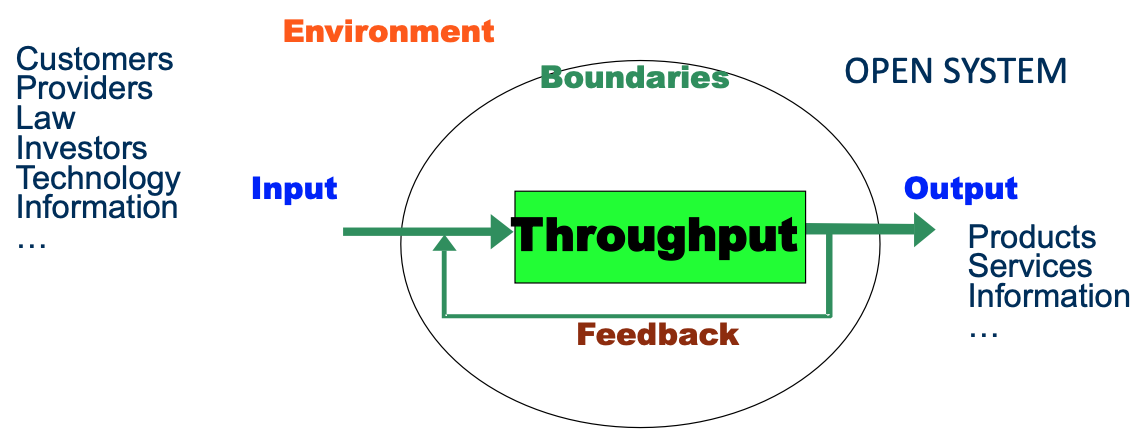
\includegraphics[width=0.7\textwidth]{fotos/1.png}
\caption{Elementos de un sistema.}
\label{fig:1}
\end{figure}

Un \textbf{sistema de información} consiste en un conjunto formal de procedimientos que, operando sobre un conjunto de datos estructurado según las necesidades de la organización, recopila, procesa, almacena y distribuye información necesaria para las operaciones diarias de la organización. Además, proporciona información a los niveles jerárquicos superiores para la toma de decisiones de acuerdo con la estrategia de negocio. \\

Es importante destacar que el objetivo de un IS es ayudar a la realización de actividades en todos los niveles de la organización, proveyendo la información correcta, con una \textbf{calidad suficiente} a la persona adecuada en el momento adecuado, en el formato más adecuado para el receptor. \\

\begin{figure}[h]
\centering
\begin{subfigure}{.5\textwidth}
\centering
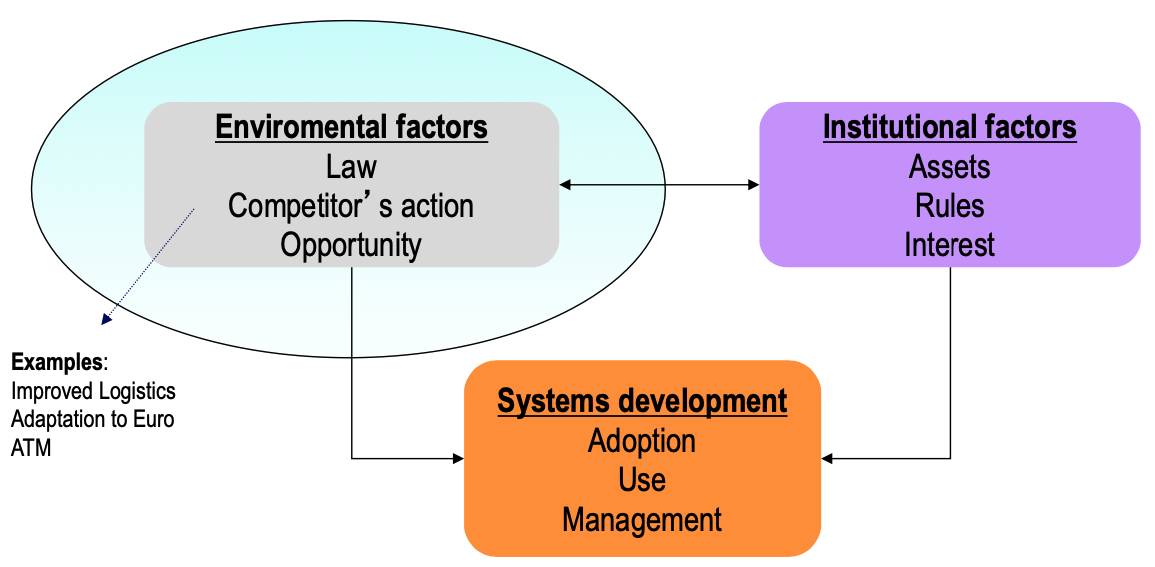
\includegraphics[width=\textwidth]{fotos/2.png}
\end{subfigure}%
\begin{subfigure}{.52\textwidth}
\centering
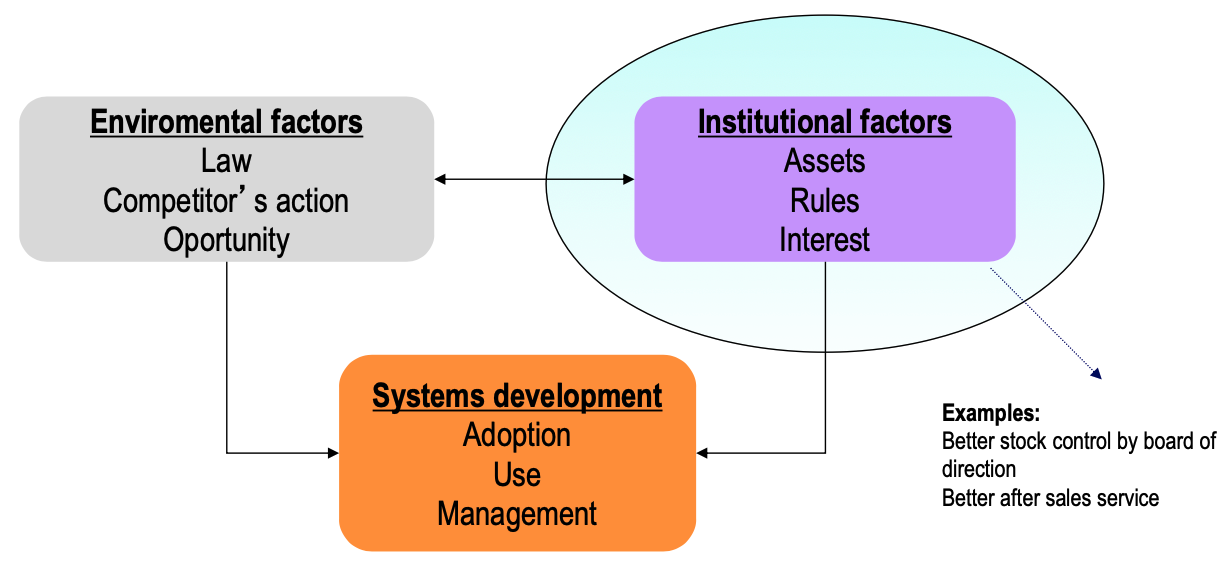
\includegraphics[width=\textwidth]{fotos/3.png}
\end{subfigure}
\caption{Sistema de información en una organización.}
\label{fig:sistema_info_org}
\end{figure}

Desde una perspectiva de negocio, un IS es una solución de organización y gestión basada en tecnología de la información, cuyo objetivo es tratar retos emergentes en el contexto del negocio. En cualquier nivel de la organización hay cambios en los objetivos, procedimientos, relaciones con el entorno, etc. para conseguir una ventaja competitiva. El valor de un IS dependerá de su efectividad, alcance, aceptación, coste, calidad de la información que produce, etc. \\

\begin{example}
\textbf{IS para la cría de mejillones.} En este caso, algunos factores ambientales serían las regulaciones regionales y nacionales, el cambio climático, los avances en tecnología, las certificaciones, el mercado, etc. Factores institucionales sería la tecnología e infraestructuras, los recursos económicos y humanos, los intereses de maximizar beneficios y expandir el mercado, etc.
\end{example}

\subsection{Sistemas de información empresarial}

Para construir un sistema de información en una empresa, se debe tener en cuenta la estrategia de negocio, lo que resulta un factor clave. A continuación habría que considerar el sistema de información a partir del cual posteriormente se obtiene la información y las tecnologías de comunicación, como sensores, algoritmos, modelos, etc. Todo esto se retroalimenta, ya que estas tecnologías muestran si la estrategia planteada es o no viable. \\

Los EIS están diseñados para coordinar el flujo de información y los registros necesarios para que una empresa funcione de manera eficiente. El sistema debe estar alineado con la estrategia empresarial de la compañía, lo que significa que la gestión de la información debe apoyat los objetivos y la dirección general del negocio. Estos sistemas ayudan a gestionar distintos aspectos de las operaciones empresariales:
\begin{itemize}
\item Planificación de recursos empresariales (ERP): integra los procesos empresariales principales en un solo sistema para garantizar una gestión eficiente de los recursos y el flujo de información.
\item Sistema de gestión de flujos de trabajo: automatizan y gestionan los procesos empresariales, asegurando que las tareas se completen en el orden correcto por las personas adecuadas.
\item Sistemas de \textit{Groupware}: herramientas que permiten a los empleados colaborar, compartir información y trabajar juntos en proyectos.
\item Sistemas de comercio electrónico. Hay tres modelos principales: business-to-business (B2B), business-to-consumer (B2C) y consumer-to-consumer (C2C).
\item Intercambio electrónico de datos (EDI): permite a las empresas intercambiar documentos comerciales en formato electrónico estandarizado.
\end{itemize}

La inteligencia de negocio ya existía antes del \textit{Big Data}. Normalmente se liga a la minería de datos, pero con la IA y los modelos predictivos, se ha ampliado su alcance. 

\subsection{Evolución de los sistemas de información}

\begin{table}[ht]
\centering
\begin{tabular}{p{1.5cm}p{3.5cm}p{3.5cm}p{4cm}}
\hline
\rowcolor{gray!50}
\textbf{Decade} & \textbf{Required Information} & \textbf{Type of ISs} & \textbf{Objectives} \\ \hline
\footnotesize 1950s & \footnotesize Basic Computational Data & \footnotesize Batch Processing Systems & \footnotesize Automate complex calculations and data processing tasks \\ \hline
\rowcolor{gray!10} \footnotesize 1960s & \footnotesize Transactional Data & \footnotesize TPS (Transaction Processing Systems) & \footnotesize Automate routine business operations and record-keeping \\ \hline
\footnotesize 1970s & \footnotesize Operational and Tactical Data & \footnotesize MIS (Management Information Systems) & \footnotesize Improve administrative control and reporting \\ \hline
\rowcolor{gray!10}\footnotesize 1980s & \footnotesize Analytical Data & \footnotesize DSS (Decision Support Systems) & \footnotesize Support decision-making with data modeling and analysis tools \\ \hline
\footnotesize 1990s & \footnotesize Strategic and Competitive Data & \footnotesize EIS (Executive Information Systems) & \footnotesize Enable real-time monitoring and strategic decision-making \\ \hline
\rowcolor{gray!10}\footnotesize 2000s & \footnotesize Enterprise-Wide Data & \footnotesize ERP (Enterprise Resource Planning Systems) & \footnotesize Integrate business functions for efficiency and process automation \\ \hline
\footnotesize 2010s & \footnotesize Big Data, Predictive Analytics & \footnotesize BI (Business Intelligence Systems) & \footnotesize Data-driven decision-making and predictive analytics \\ \hline
\rowcolor{gray!10}\footnotesize 2020s & \footnotesize Real-Time and AI-Enhanced Data & \footnotesize AI Systems and Cloud-Based Analytics & \footnotesize Automate decisions with AI, scalable cloud infrastructure \\ \hline
\end{tabular}
\caption{Evolution of Information Systems by Decade}
\end{table}

\subsection{Tipos de sistemas de información}

\begin{itemize}
\item Sistemas de nivel operacional. Monitorizan las actividades, operaciones y transacciones básicas de la empresa. 
\item Sistemas de gestión de informacion (MIS) y sistemas de soporte de decisión (DSS). Ayudan la monitorización, control y toma de decisiones y actividades administrativas a nivel gerencial. 
\item Sistemas de nivel estratégico. Apoyan la planificación a largo plazo a nivel gerencial para lograr una ventaja competitiva.
\item Sistemas de nivel de conocimiento. Apoyan a los trabajadores de conocimiento e información dentro de la institución.
\end{itemize}

\begin{example}
\textbf{USC:}
\begin{itemize}
\item Operacional: inscripciones de estudiantes.
\item MIS: informes mensiales sobre el desempeño estudiantil.
\item DSS: análisis de tendencias en la inscripción de estudiantes.
\item Estratégico: decisiones a largo plazo sobre nuevos grados y líneas de investigación.
\item Conocimiento: repositorio digital con tesis, artículos e investigaciones.
\end{itemize}
\end{example}

\subsubsection{Sistemas de información operacional}

Las características principales de estos sistemas son:
\begin{itemize}
\item Ejecutan y registran operaciones rutinarias diarias necesarias para el funcionamiento de la empresa. 
\item Diseñados para aumentar la productividad.
\item La inversión en estos sistemas es fácil de justificar ante la dirección, ya que sus beneficios son viables y palpables. 
\item Comúnmente, son el primer tipo de IS que se implementa en una empresa. Su uso inicial apoya los esfuerzos a nivel operacional.
\item Son intensivos en entrada y salida de datos. Las operaciones que realizan generalmente implican cálculos y procesos simples y poco sofisticados. 
\item Proporcionan a los administradores informes y acceso en línea a registros históricos y diarios.
\item Son los principales generadores de información para otros tipos de ISs dentro de la organización.
\end{itemize}

Como ejemplos de OIS se pueden comentar sistemas de facturación, sistemas de control de inventario o sistemas que calculan y procesan los pagos de los empleados. 

\subsubsection{Sistemas de soporte de decisión}

Las características principales de estos sistemas son:
\begin{itemize}
\item Se incluyen tras haber implementado IS más relevantes, ya que reciben información de estos sistemas.
\item Los cálculos suelen ser intensivos, mientras que las salidas son escasas. 
\item Combinan información cambiante con modelos analíticos sofisticados para apoyar la toma de decisiones no estructurada y semiestructurada. 
\item Tienden a ser interactivos, visuales y amigables, y están enfocados en el usuario final.
\item No tienen la intención de ahorrar trabajo. Como resultado, la justificación económica para la inversión en estos sistemas es dificil, ya que no se conocen los beneficios directos del proyecto. 
\item Involucran modelos analíticos, análisis de ``qué pasaría si'', simulaciones y pronósticos.
\end{itemize}

\subsubsection{Sistemas estratégicos}

Las características principales de estos sistemas son:
\begin{itemize}
\item Incorporan información externa y obtienen información resumida de los sistemas operacionales y de soporte de decisión.
\item Apoyan la introducción de productos y procesos dentro de la organización, ya que buscan obtener una ventaja sobre los competidores mediante innovación.
\item Si función es lograr ventajas que los competidores no tienen, como ventaja de costos y servicios diferenciados para clientes y proveedores. En este contexto, los sistemas estatégicos crean barreras de entrada para el negocio. Por ejemplo los cajeros automáticos (ATM), la banca por internet y los sistemas de recomendación.
\item Suelen desarrollarse de forma ad hoc dentro de la organización.
\item Están orientados a alcanzar metas estratégicas a largo plazo (e.g. expandir la cuota de mercado, crear nuevos mercados).
\end{itemize}

Como ejemplos de SIS se pueden comentar pronósticos de ventas (con planificación de campañas de marketing), planificación de recursos de manufactura (MRP) enfocado en aumentar la productividad en un proceso de manufactura, descubrimiento y lanzamiento de productos en banca, como tipos de hipoteca, con el propósito de alcanzar objetivos comerciales tales como atraer nuevos clientes o fidelizar a los actuales, etc.

\begin{table}[ht]
\centering
\begin{tabular}{p{2.75cm}p{2.5cm}p{3cm}p{2.5cm}p{2.5cm}}
\hline
\rowcolor{gray!50}
\textbf{Sistema} & \textbf{Entrada} & \textbf{Procesos} & \textbf{Salida} & \textbf{Usuarios} \\ \hline
\footnotesize Operacional & \footnotesize Transacciones & \footnotesize Almacenar, informar, unir & \footnotesize Informes, resúmenes, transacciones, facturas, nóminas. & \footnotesize Personal operativo, supervisor \\ \hline
\footnotesize DSS, táctico & \footnotesize Información operacional resumida, gran volumen de datos, modelos simples & \footnotesize Modelo, simulaciones, análisis, optimización, análisis de "qué pasaría si"  & \footnotesize Informes analíticos, modelos de decisión & \footnotesize Personal técnico, analístas de datos \\ \hline
\footnotesize Sistemas estratégicos & \footnotesize Información agregada, información externa & \footnotesize Análisis estratégico, planificación de escenario, CI & \footnotesize Planes estratégicos, predicciones & \footnotesize Directiva \\ \hline
\end{tabular}
\caption{Características de distintos IS.}
\end{table}

\section{Inteligencia de negocio}

El término ``inteligencia de negocio'' (BI) se refiere a la gestión de la información en una empresa específica o área de negocio. Conciste en un conjunto de estrategias y herramientas focalizadas en la gestión del conocimiento mediante el análisis de los datos de la organización. BI se centra en:
\begin{itemize}
\item Marcar objetivos de negocio.
\item Determinar la necesidad de datos, información y conocimiento para complir los objetivos.
\item Hay que \textbf{integrar} todos esos daots con toda esa información, deben ser accesibles y fundamentar decisiones.
\end{itemize}

Como ya se vio antes, los OIS recogen y organizan los datos, los IS tácticos la analizan, resumen, transforman y visualizan, mientras que los SIS adquieren, descubren, evalúan y usan ese conocimiento generado a partir de los datos. 

\begin{figure}[h]
\centering
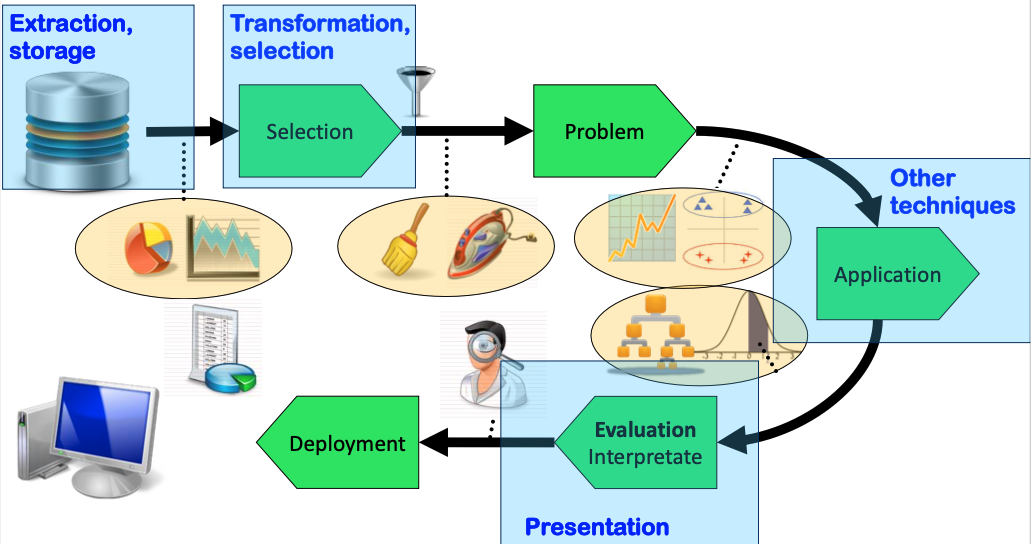
\includegraphics[width=0.75\textwidth]{fotos/4.png}
\caption{Proceso de inteligencia de negocio. Para su aplicación se puede usar minería de datos u otras técnicas.}
\label{fig:4}
\end{figure}

\section{Modelos de madurez}

Los modelos de madurez (MM) permiten evaluar el nivel de desarrollo y eficacia en el uso de soluciones, así como formas de mejora. Definen niveles de definición, eficiencia, manejabilidad y medición del entorno monitoreado. Generalmente todos siguen una estructura similar, y tienen las siguientes características comunes: 
\begin{itemize}
\item Cada modelo tiene al menos 5 niveles de madurez; menos implica pasar de fases de forma confusa. 
\item Cada modelo empieza con una fase primitiva
\item Los modelos no se centran solo en la tecnología, se basan también en el involucramiento de las personas y los procesos.
\item Proporcionan capacidades actuales, hojas de ruta para la mejora, comparación de referencias, alineación con los objetivos empresariales, mejoran la cultura basada en datos, optimizar la asignación de recursos y apoyar la planificación estratégica.
\end{itemize}

\subsection{The Data Warehousing Institute (TDWI) Analytics MM}
Este modelo consta de las siguientes dimensiones: 
\begin{center}
    % Primera fila con tres columnas
    \begin{minipage}{0.3\textwidth}
        \begin{tcolorbox}[colback=red!25, colframe=red!75, width=5cm, height=5cm, title=Madurez Organizacional, fonttitle=\color{black}\bfseries, valign=center, left=1mm, right=1mm, arc=2mm, boxrule=0.5mm]
            \begin{itemize}
                \item Liderazgo
                \item Cultura
                \item Impacto
                \item Estrategia
            \end{itemize}
        \end{tcolorbox}
    \end{minipage} \hfill
    \begin{minipage}{0.3\textwidth}
        \begin{tcolorbox}[colback=orange!25, colframe=orange!75, width=5cm, height=5cm, title=Madurez de Recursos, fonttitle=\color{black}\bfseries, valign=center, left=1mm, right=1mm, arc=2mm, boxrule=0.5mm]
            \begin{itemize}
                \item Financiamiento
                \item Talento / habilidades
                \item Roles / responsabilidades
                \item Capacitación
            \end{itemize}
        \end{tcolorbox}
    \end{minipage} \hfill
    \begin{minipage}{0.3\textwidth}
        \begin{tcolorbox}[colback=brown!25, colframe=brown!75, width=5cm, height=5cm, title=Madurez de la Infraestructura de Datos, fonttitle=\color{black}\bfseries, valign=center, left=1mm, right=1mm, arc=2mm, boxrule=0.5mm]
            \begin{itemize}
                \item Diversidad, volumen y velocidad
                \item Acceso a datos
                \item Integración y gestión de datos
                \item Arquitectura de datos
            \end{itemize}
        \end{tcolorbox}
    \end{minipage}
\end{center}
\begin{center}
    % Segunda fila con dos columnas
    \hspace{1.65cm}
    \begin{minipage}{0.45\textwidth}
        \begin{tcolorbox}[colback=green!25, colframe=green!75, width=5.5cm, height=5.5cm, title=Madurez Analítica, fonttitle=\color{black}\bfseries, valign=center, left=1mm, right=1mm, arc=2mm, boxrule=0.5mm]
            \begin{itemize}
                \item Alcance de capacidades
                \item Automatización / aumentar
                \item Enfoques de despliegue y entrega
                \item Innovación
            \end{itemize}
        \end{tcolorbox}
    \end{minipage} \hspace{-1.25cm}
    \begin{minipage}{0.45\textwidth}
        \begin{tcolorbox}[colback=cyan!25, colframe=cyan!75, width=5.5cm, height=5.5cm, title=Madurez de Gobernanza, fonttitle=\color{black}\bfseries, valign=center, left=1mm, right=1mm, arc=2mm, boxrule=0.5mm]
            \begin{itemize}
                \item Procesos y herramientas de gobernanza de datos
                \item Procesos y herramientas de gobernanza del modelo
                \item Roles de gobernanza
                \item Seguridad/privacidad
            \end{itemize}
        \end{tcolorbox}
    \end{minipage}
\end{center}

Entre la tercera y cuarta etapa, hay un abismo que muchas empresas no llegan o no quieren cruzar. Las fases del modelo son las siguientes: 

\begin{table}[h]
\centering
\begin{tabular}{p{15cm}}
    \hline
    \rowcolor{gray!10} Etapa 1: Naciente - Entorno pre-analítico. La cultura no está basada en datos y no se toman decisiones basadas en datos. No hay una infraestructura formal de BI. Los datos están dispersos y en silos. Calidad pobre de datos. IT y negocio no trabajan juntos. Informes en Excel o manuales. \\ \hline
    
    Etapa 2: Temprana - Herramientas básicas de BI. Comenzando a entender el valor de la analítica. La organización se da cuenta de que se necesita cierta infraestructura de datos para apoyar la integración de datos para el análisis. Analítica rudimentaria pero en avance. Calidad de los datos inconsistente ya que nadie se ocupa de ellos. \\ \hline
    
    \rowcolor{gray!10} Etapa 3: Establecida - Se ha implementado un data warehouse. Hay un grupo responsable de la analítica en IT. Se ha formado un equipo de gobernanza de datos. Se utilizan herramientas de visualización de datos. La solución no escala bien y no hay aún herramientas de fácil uso. \\ \hline
    
    Etapa 4: Madura - Los usuarios finales integran la analítica en la toma de decisiones y operaciones. Cultura de innovación y colaboración entre IT y negocio. Uso de diversas fuentes, incluidos datos semi y no estructurados. La fuerza laboral incluye científicos de datos, ingenieros de datos, MLOps y roles como el Chief Analytics Officer. \\ \hline
    
    \rowcolor{gray!10} Etapa 5: Avanzada / Visionaria - Analítica de autoservicio. La organización considera la analítica como un arma competitiva crítica. Infraestructura operativa, flexible y escalable (data lakes, DWH, nube), ML, AI se utiliza en NRT para la toma de decisiones. \\ \hline
\end{tabular}
\end{table}

Esta organización proporciona un test para evaluar el nivel de madurez de una empresa u organización en BI, dando una visión holística: es de esperar que que las fases varíen para cada dimensión.

\begin{figure}[h]
\centering
\begin{subfigure}{.4078\textwidth}
\centering
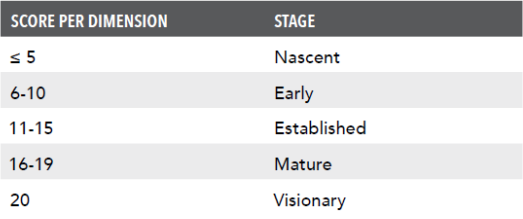
\includegraphics[width=\textwidth]{fotos/5.png}
\end{subfigure}%
\begin{subfigure}{.5922\textwidth}
\centering
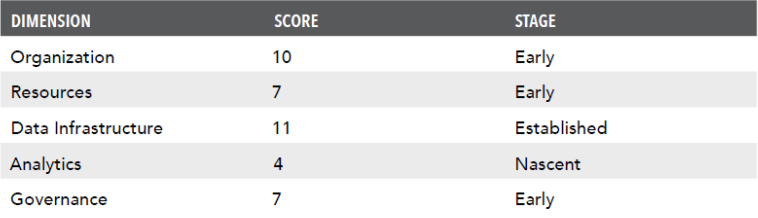
\includegraphics[width=\textwidth]{fotos/6.png}
\end{subfigure}
\caption{Test de madurez de TDWI: resultados.}
\label{fig:tdwi}
\end{figure}

\subsection{HP BI MM}

\begin{table}[H]
\centering
\begin{tabular}{p{15cm}}
    \hline
    \rowcolor{gray!10} Etapa 1: Operación (Operar el negocio) - Implica soluciones ad-hoc enfocadas en la demanda local. No existe una estrategia formal de BI ni analítica. \\ \hline
    
    Etapa 2: Mejora (Medir y monitorear el negocio) - BI más estructurado. Se está utilizando la analítica. Los almacenes de datos (DW) aún están enfocados en unidades de negocio específicas. \\ \hline
    
    \rowcolor{gray!10} Etapa 3: Alineación - BI alineado con los objetivos estratégicos. Integración de la información entre áreas temáticas. La calidad de los datos y la gobernanza están aumentando su importancia. La organización ha evolucionado de la gestión de proyectos de BI a la gestión de programas de BI. \\ \hline
    
    Etapa 4: Empoderamiento - Se utilizan herramientas de autoservicio a todos los niveles. Se implementan análisis avanzados. Existe una única versión de la verdad en toda la organización. BI es fundamental. \\ \hline
    
    \rowcolor{gray!10} Etapa 5: Excelencia (Cambiar el negocio) - Análisis predictivo para la mayoría de las decisiones empresariales. Arquitectura orientada a servicios (SOA) para la entrega de información. Los análisis se entregan rápidamente a los usuarios. \\ \hline
\end{tabular}
\end{table}

En este modelo de 5 etapas de madurez, el éxito se contempla como una función de cada una de las dimensiones: habilitación/preparación del negocio, gestión de la información, estrategia y programa de gestión.

\begin{figure}[h]
\centering
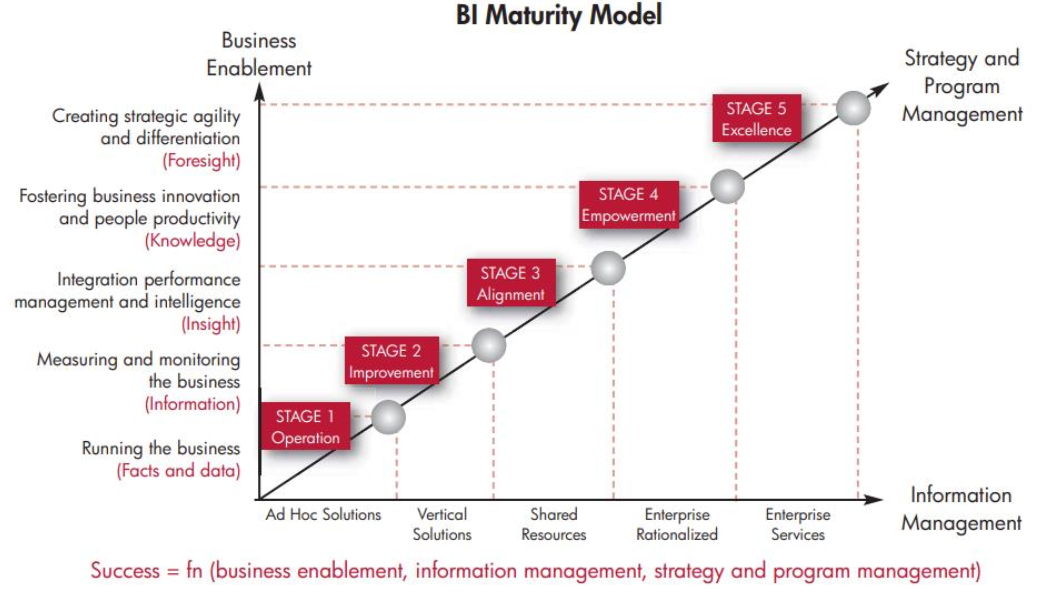
\includegraphics[width=0.9\textwidth]{fotos/7.png}
\caption{Modelo de madurez de BI de HP.}
\label{fig:7}
\end{figure}

\subsection{Gartner BI MM}

\begin{figure}[H]
\centering
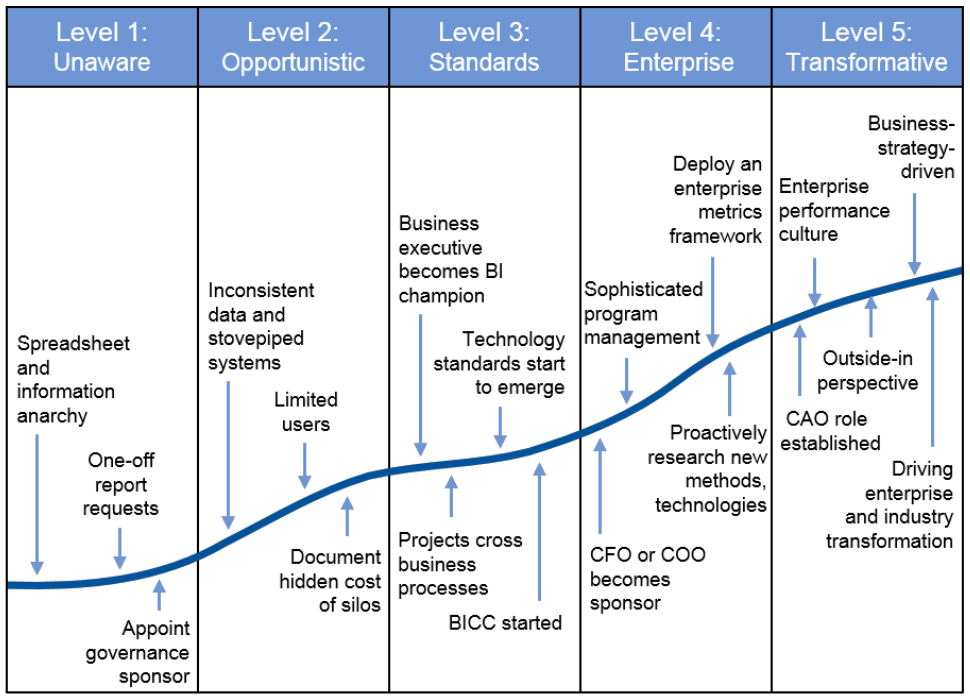
\includegraphics[width=0.9\textwidth]{fotos/8.png}
\caption{Modelo de madurez de BI de Gartner (BICC - \textit{BI competency center}).}
\label{fig:8}
\end{figure}

Este se trata de un modelo popular, que tiene muy en cuenta el entorno de la organización a la hora de tomar decisiones (\textit{external drivers}). En la primera etapa no se usa BI. En la segunda se empiezan a compartir datos. En la tercera no hay interacción entre las unidades de negocio. En la cuarta, existen políticas y estándares bien definidos y en última etapa, la información es confiable y se tiene una solución adaptable a las entidades de la empresa. 

\begin{table}[h]
\centering
\begin{tabular}{p{15cm}}
    \hline
    \rowcolor{gray!10} Nivel 1: Desconocido - BI y analítica ad-hoc. No hay un proceso formal de toma de decisiones. No hay infraestructura de TI. \\ \hline
    
    Nivel 2: Oportunista - Las unidades de negocio usan BI de forma individual. Cada proyecto/unidad tiene su propia infraestructura. \\ \hline
    
    \rowcolor{gray!10} Nivel 3: Estandarizado - La coordinación mejora. Proyectos que abarcan múltiples procesos de negocio. Se crea un centro de competencia de BI. Empiezan a surgir estándares tecnológicos para la infraestructura, DW y plataformas de BI. \\ \hline
    
    Nivel 4: Empresarial - Los altos ejecutivos patrocinan BI. Se han definido métricas de rendimiento que guían la estrategia. BI apoya los procesos de decisión en toda la empresa. \\ \hline
    
    \rowcolor{gray!10} Nivel 5: Transformador - BI y la analítica son una iniciativa estratégica gestionada y apoyada por el negocio y TI. Se utilizan para generar ingresos. Usuarios en todos los niveles, incluidos clientes y socios. \\ \hline
\end{tabular}
\end{table}


\section{Metodología}

El primer paso en la implementación de BI es desarrollar una declaración clara del problema. Todo proceso debe ser repetible (esto hará más fácil su asimilación). Los procesos, creados por expertos, ayudan a la planificación y gestión de procesos. Además, reduce el miedo inicial a afrontar el problema, ya que existe un proceso estandarizado y reduce la dependencia en personal específico. Como ejemplos de metodologías se pueden mencionar:
\begin{itemize}
\item Gestión: PMBok, Agile, ... 
\item Gestión y desarrollo: Larissa, Kimball, Inmon, SAFE, QPM (QlikView), ASAP (SAP), ...
\item CRISP-DM: tareas genéricas para minería de datos (DM).
\begin{itemize}
    \item Procesos estandarizados intersectoriales para DM.
    \item Propuestos por un consorcio (SPSS, NCR, AG, OHRA).
    \item Otras metodologías centradas en DM podrían ser: 5A'S, critikal, CAT (Clementine Application Template), SEMMA (SAS, Sample, Explore, Modify, Model, Assess), ... 
\end{itemize}
\end{itemize}

\subsection{Larissa Moss}

\begin{minipage}{0.4\textwidth}
    \centering
    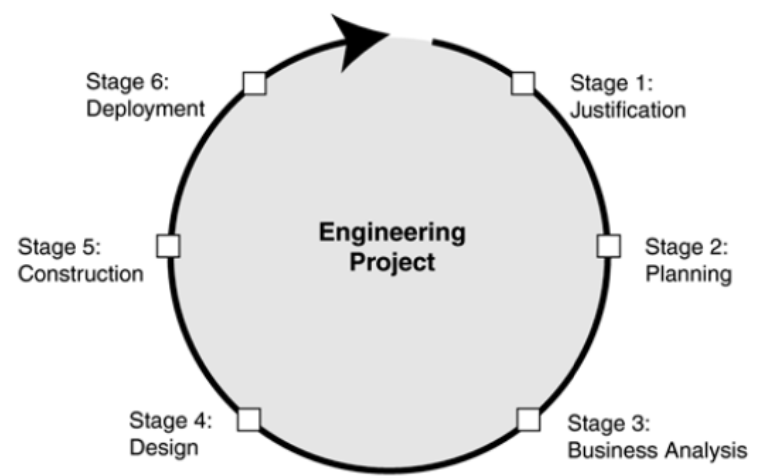
\includegraphics[width=\linewidth]{fotos/10.png} 
\end{minipage} \hfill
\begin{minipage}{0.6\textwidth}
    Este modelo define una hoja de ruta con 6 etapas iterativas y 16 pasos.  \\

    Define etapas, pasos, cargos, estándares y entregable. Es ágil y flexible, además de promocionar subproyectos, ya que fragmenta los proyectos grandes. Veamos un desglose de las etapas y los pasos a seguir en cada una de ellas:
\end{minipage}


\begin{minipage}{0.4\textwidth}
    \centering
    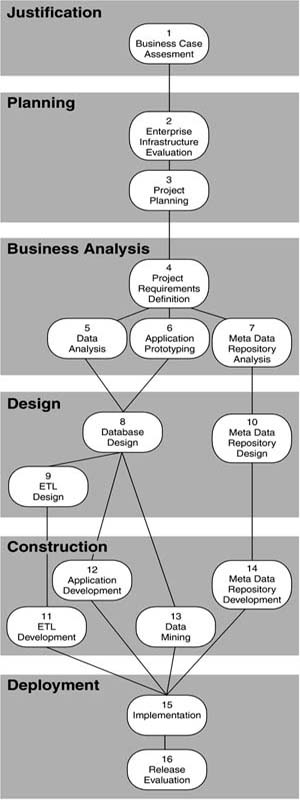
\includegraphics[width=\linewidth]{fotos/11.png} 
\end{minipage} \hfill
\begin{minipage}{0.6\textwidth}
\begin{enumerate}
\item Justificación: evaluar la necesidad empresarial que da lugar al nuevo proyecto de ingeniería.
\begin{itemize}
\item Paso 1. Evaluación del caso de negocio.
\begin{itemize}
\item Define el problema u oportunidad empresarial y propone una solución de BI.
\item Cada lanzamiento de aplicación de BI debe estar justificado en costos y debe definir claramente los beneficios.
\end{itemize}
\end{itemize}
\item Planificación: desarrollar planes estratégicos y tácticos, que establezcan cómo se llevará a cabo y desplegará el proyecto de ingeniería.
\begin{itemize}
\item Paso 2. Evaluación de la infraestructura empresarial.
\begin{itemize}
\item Técnico: hardware, software, redes, ... 
\item No técnico: procedimientos, metodologías, ...
\end{itemize}
\item Paso 3. Planificación del proyecto: alcance, personal, presupuesto, tecnología, representantes empresariales, ...
\end{itemize}
\item Análisis de negocio: realizar un análisis detallado del problema u oportunidad empresarial para obtener una comprensión sólida de los requisitos del negocio para una solución potencial (producto).
\begin{itemize}
\item Paso 4. Definición de requisitos del proyecto.
\begin{itemize}
\item Gestión y especificación del alcance, necesidades del usuario, ...
\item Se entrega el \textit{Service Level Agreement} (SLA).
\end{itemize}
\item Paso 5. Análisis de datos, disponibilidad, calidad, ...
\end{itemize}
\end{enumerate}
\end{minipage}

\begin{enumerate}
\setcounter{enumi}{3}
\item[] \quad 
\begin{itemize}
\item Paso 6. Prototipado de la aplicación. Ayuda en la definición de requisitos y evita riesgos.
\item Paso 7. Análisis del repositorio de metadatos.
\begin{itemize}
\item Los metadatos técnicos deben ser mapeados a los metadatos del negocio. 
\item Los metadatos describen una organización en términos de sus actividades comerciales, los objetos del negocio y las reglas bajo las cuales se realizan las actividades comerciales (e.g. definiciones, unidades, relaciones, fuentes, ...)
\end{itemize}
\end{itemize}
\item Diseño: concebir un producto que resuelva el problema empresarial o permita la oportunidad empresarial.
\item Construcción: construir el producto, el cual debe proporcionar un retorno de inversión dentro de un periodo de tiempo predefinido.
\item Despliegue: implementar o vender el producto terminado, y luego medir su efectividad para determinar si la solución cumple, excede o no cumple con el retorno de inversión esperado.
\end{enumerate}

\subsection{CRISP-DM}

Esta metodología es libre e independiente de aplicación, contexto y herramientas. Se trata de una guía que considera el problema y las técnicas, y está basado en la experiencia. Hay 2 documentos principales: el modelo de referencia, que describe las fases, tareas y salidas, y la guía de usuario, con consejos de aplicación práctica, listas, etc. CRISP-DM es el proceso más usado para proyectos de ciencia de datos. \\

\begin{figure}[h]
\centering
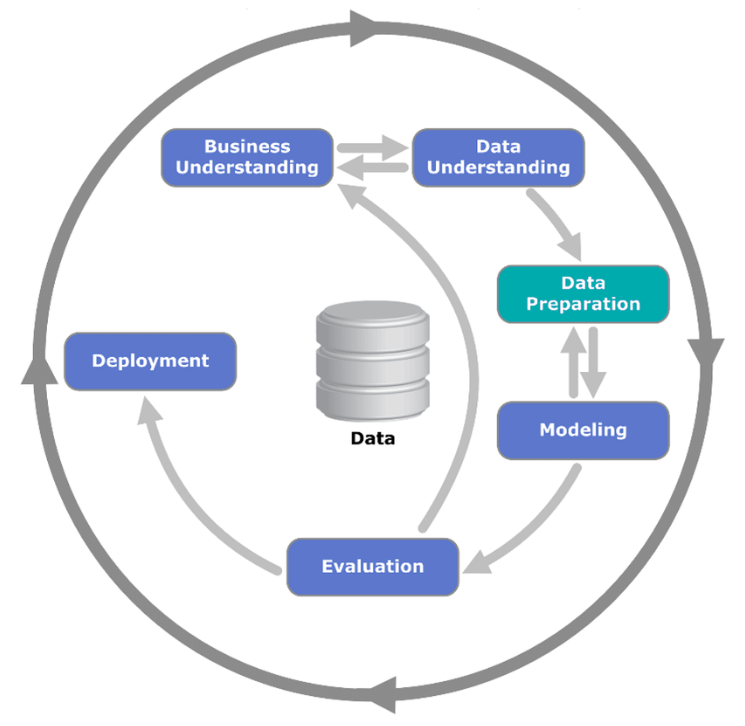
\includegraphics[width=0.6\textwidth]{fotos/12.png}
\caption{Fases de CRISP-DM.}
\label{fig:12}
\end{figure}

Hay 4 niveles de jerarquía: las fases se dividen en tareas generales, estas se fragmentan en tareas específicas que a su vez de dividen en instancias de proceso. La metodología se compone de 6 fases bien diferenciadas; las 3 primeras representan de forma general el 80\% de un proyecto de ciencia de datos (30\% entre las fases 1 y 2 y 50\% para la fase 3): 

\begin{figure}[H]
\centering
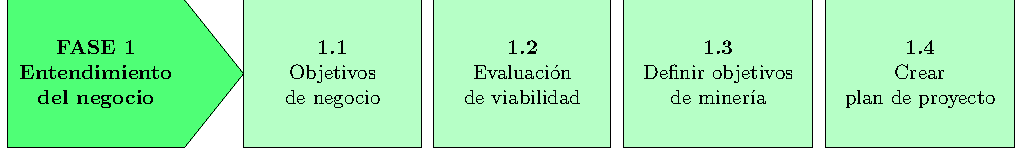
\includegraphics[width=\textwidth]{fotos/13.pdf}
\end{figure}

Un gran fallo es considerar que comprender el negocio es un objetivo secundario; se trata de uno de los aspectos más importantes. Se tienen las siguientes tareas:
\begin{enumerate}[label=1.\arabic*]
\item Definir los objetivos del negocio. 
\begin{itemize}
\item Conocer lo que quiere el cliente desde la perspectiva del negocio: ¿mejorar la gestion de inventario?, ¿reducir el tiempo de respuesta?, ¿mejorar la calidad de los productos?, ...
\item Mostrar los factores que afecten al proyecto.
\item Establecer el criterio de éxito.
\end{itemize}
\item Evaluación de viabilidad. Es común usar análisis DAFO (debilidades, amenazas, fortalezas, oportunidades) para evaluar la viabilidad del proyecto.
\begin{itemize}
\item Indicar recursos (personal, datos, \textit{software}, ...), restricciones, suposiciones, requerimientos y otros factores como el hecho de si tenemos permitido usar los datos.
\item Evaluación del costo-beneficio.
\item Riesgos: no disponibilidad de los datos, conocimiento no disponible, herramientas
\end{itemize}
\item Definir los objetivos de minería.
\begin{itemize}
\item Objetivos específicos del problema: traducir las necesidades del cliente en objetivos de minería mediante segmentación, patrones secuanciales, ... 
\item Establecer objetivos técnicos: traducir las metas en parámetros de salida, como el ratio de éxito, predicciones de fracaso, coste de error, etc.
\end{itemize}
\item Crear un plan de proyecto.
\begin{itemize}
\item Establecer los pasos: la duración, los recursos necesarios, las entradas y las salidas. Organizar y gestionar riesgos. 
\item Elección inicial de herramientas y técnicas.
\end{itemize}
\end{enumerate}

\begin{figure}[H]
\centering
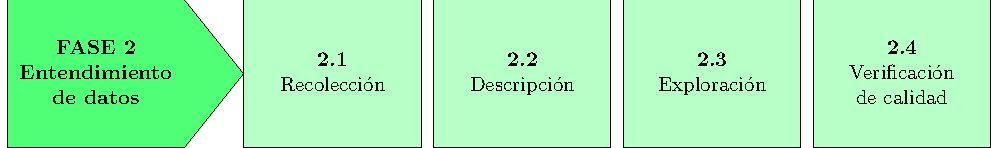
\includegraphics[width=\textwidth]{fotos/14.pdf}
\end{figure}

\begin{enumerate}[label=2.\arabic*]
\item Recolección: definir las fuentes, integración (suele ser la parte más complicada), localización, problemas y soluciones, etc.
\item Descripción: formato, claves, cantidad, etc.
\item Exploración: consultas, visualización, informes, distribución de valores, agregaciones de datos, estadísticas, etc.
\item Verificación de calidad: ¿todos los tipos de datos?, ¿todas las clases representadas?, ¿suficientes datos?, ¿datos completos?, ¿valores nulos o anormales?, etc.
\end{enumerate}


\begin{figure}[H]
\centering
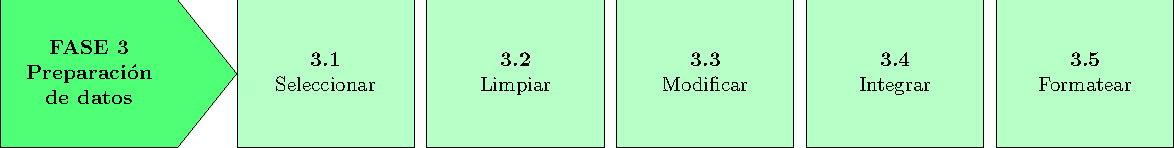
\includegraphics[width=\textwidth]{fotos/15.pdf}
\end{figure}

\noindent Esta fase supone un 50\% del tiempo total del proyecto.

\begin{enumerate}[label=3.\arabic*]
\item Selección de datos.
\begin{itemize}
\item Seleccionar tablas, atributos y filas.
\item Volumen adecuado para las herramientas.
\item Selección: dividir el conjunto de datos en \textit{training}, \textit{test} y \textit{validation}.
\item Muestra de datos (\textit{samples}).
\end{itemize}
\item Limpiar daots incompletos o erróneos.
\begin{itemize}
\item Mejorar la calidad de los datos.
\item Seleccionar un subconjunto de datos, reemplazar valores nulos.
\item Completar, eliminar o ignorar valores.
\end{itemize}
\item Transformación.
\begin{itemize}
\item Elegir los atributos más relevantes.
\item Derivar las nuevas características más significativas a partir de las originales.
\item Discretización, \textit{mapear}, normalizar, ...
\end{itemize}
\item Integrar: almacén de datos (\textit{datawarehouse}).
\item Formatear: si es necesario para las técnicas posteriores. Conocido como ETL (extracción, transformación y carga).
\begin{itemize}
\item Normalmente usa un modelo gráfico. Involucra la monitorización de la ejecución, el grabado de los datos y excepciones y errores.
\end{itemize}
\end{enumerate}

\begin{figure}[H]
\centering
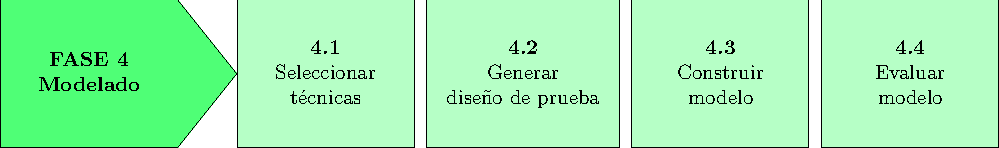
\includegraphics[width=\textwidth]{fotos/16.pdf}
\end{figure}

Para la descripción de esta fase, se asume una vista minable: una tabla que contenga los atributos relevantes, etiquetados como entradas y salidas. 

\begin{enumerate}[label=4.\arabic*]
\item Técnicas de selección, considerando:
\begin{itemize}
\item Adecuación al problema: clasificación, predicción, agrupamiento, asociación, dependencias, ...
\item Con datos adecuados.
\item Cumpliento con los requisitos del problema.
\item Ejecutable a tiempo. 
\item Conocimiento de la técnica.
\end{itemize}
\item Diseños de test.
\begin{itemize}
\item Establecer \textit{training}, \textit{testing} y \textit{validation}.
\item Establecer criterios para la bondad del modelo. 
\end{itemize}
\item Crear el modelo: fijar los parámetros y ejecutarlo.
\item Evaluar el modelo: ¿cumple con la calidad esperada? 
\end{enumerate}

\begin{figure}[H]
\centering
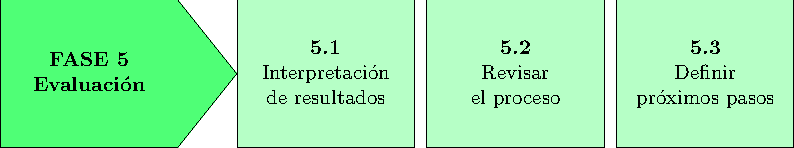
\includegraphics[width=0.8\textwidth]{fotos/17.pdf}
\end{figure}

\begin{enumerate}[label=5.\arabic*]
\item Interpretar los resultados: ¿queda resuelto el problema?, ¿es apropiada la respuesta?, ¿es válida?, ¿está bien definido el objtivo del negocio?, ¿es un conocimiento nuevo?, ¿es útil el modelo?, ¿es mejor que lo que se tenía antes?, ¿hay muchos patrones?, ... 
\item Revisar el proceso: ¿algún error desde el punto de vista técnico?, ¿se ha pasado algo por encima?
\item Definir los siguientes pasos: ¿iterar?, ¿desplegar?, ¿reconstruir?, ...
\end{enumerate}

\begin{figure}[H]
\centering
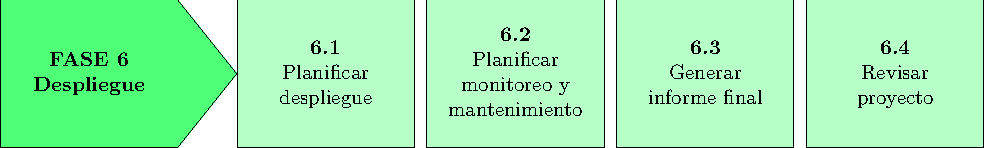
\includegraphics[width=\textwidth]{fotos/18.pdf}
\end{figure}

\begin{enumerate}[label=6.\arabic*]
\item Planificación del despliegue: ¿quiénes son los usuarios?, ¿cómo y cuándo será usado el modelo?, ¿cómo será desplegado?, ¿cómo una herramienta?, ¿es necesario un programa de ordenador?, ... 
\item Planificación del seguimiento y mantenimiento: ¿se está usado?, ¿se está usando de forma adecuada?, ¿modelos actualizables?, ...
\item Generar un informe final.
\item Revisar el proyecto: debilidades y fortalezas, aspectos a mejorar, ...
\end{enumerate}